Il presente capitolo illustra i paradigmi architetturali e le tecnologie che costituiscono le fondamenta del lavoro di tesi. La ratio logica di questa sezione segue un approccio top-down: si analizzano inizialmente i pattern architetturali distribuiti per giustificare la scelta del modello Serverless; successivamente, si esamina lo specifico stack tecnologico offerto da Amazon Web Services (AWS) per l'implementazione di tali pattern; infine, si descrivono gli strumenti di automazione e le metodologie operative necessari per gestire in modo rigoroso l'infrastruttura e il ciclo di sviluppo.

\section{Architetture Distribuite e Cloud Computing}
\label{sec:cloud_arch}

L'ingegneria del software moderna privilegia l'adozione di sistemi distribuiti e modulari rispetto alle tradizionali architetture monolitiche, al fine di garantire una maggiore tolleranza ai guasti e un'allocazione scalabile delle risorse.

\subsection{Il modello a Microservizi: vantaggi e complessità operativa}
L'architettura a microservizi scompone un'applicazione in un insieme di servizi indipendenti, ciascuno eseguito in un proprio processo e comunicante tramite protocolli leggeri, tipicamente API HTTP, come formalizzato da Dragoni et al. \cite{MicroservicesDragoni}. Questa suddivisione, illustrata in Figura \ref{fig:monovsmicro}, consente lo scaling orizzontale dei singoli componenti e disaccoppia i cicli di sviluppo dei vari team. 
La letteratura scientifica concorda nell'affermare che tale paradigma introduce un elevato grado di complessità operativa \cite{FowlerMicroservices}. Nello specifico, la gestione di chiamate di rete, il mantenimento della consistenza dei dati in sistemi distribuiti e l'orchestrazione del deployment di molteplici unità indipendenti richiedono infrastrutture di automazione rigorose.

\begin{figure}[ht!]
    \centering
    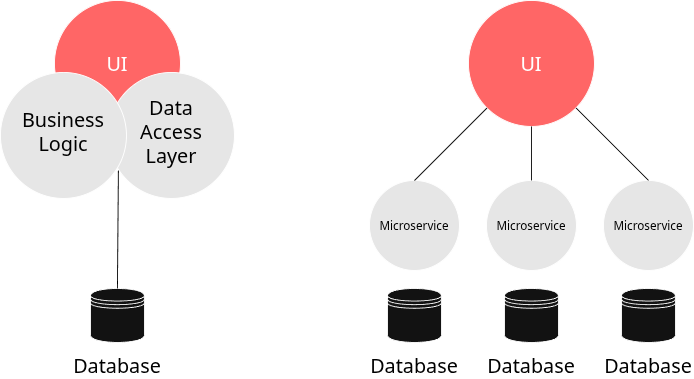
\includegraphics[width=1\textwidth]{images/monolitevsmicro.drawio.png}
    \caption{Confronto strutturale tra architettura Monolitica e a Microservizi [Elaborazione dell'autore]}
    \label{fig:monovsmicro}
\end{figure}

\subsection{Serverless Computing e Function-as-a-Service (FaaS)}
Il Serverless Computing delega al fornitore Cloud la completa gestione dell'allocazione e del provisioning delle risorse computazionali. Come definito da Jonas et al. \cite{BerkeleyServerless}, questo modello combina servizi di backend gestiti con il paradigma Function-as-a-Service (FaaS).
L'operatore fornisce il codice sorgente sotto forma di funzioni, le quali vengono eseguite esclusivamente in reazione a specifici eventi. Questo approccio elimina la manutenzione dei server virtuali e introduce un modello di tariffazione basato sul consumo reale: i costi derivano dal tempo di esecuzione, misurato in millisecondi, e dalla memoria allocata, differenziandosi dai modelli basati sulla disponibilità fissa delle istanze \cite{EC2}.
L'infrastruttura Serverless risulta particolarmente indicata per la gestione di carichi di lavoro discontinui. La presenza di piani tariffari gratuiti per i bassi volumi di traffico consente inoltre di mantenere i costi infrastrutturali prossimi allo zero per gli ambienti di test e per ambienti a basso carico \cite{EivyEconomics}.

\section{Stack Tecnologico per High-Throughput su AWS}
\label{sec:aws_stack}

Amazon Web Services (AWS) eroga una suite di servizi per l'implementazione di architetture Serverless. La selezione di tale fornitore si basa sull'integrazione nativa tra i componenti di calcolo, archiviazione ed elaborazione dati.

\subsection{Compute Layer: AWS Lambda}
AWS Lambda è il servizio di calcolo guidato da eventi che esegue la logica applicativa dell'architettura proposta. Nei sistemi event-driven, il flusso di esecuzione è innescato da variazioni di stato, come il caricamento di un file o la ricezione di una richiesta di rete \cite{EventDrivenArchitecture}.

Le funzioni Lambda sono definite da due proprietà tecniche fondamentali. La prima è l'assenza di stato (stateless): l'ambiente di esecuzione non conserva memoria delle invocazioni precedenti, rendendo necessario l'utilizzo di servizi di storage esterni per la persistenza dei dati.
La seconda proprietà riguarda l'effimerità dell'ambiente di calcolo. Il container che ospita il codice viene istanziato al verificarsi dell'evento e sospeso o terminato al completamento dell'esecuzione. Questa dinamica introduce il fenomeno noto come Cold Start, visibile in Figura \ref{fig:lambda_cold_start}, ovvero una latenza aggiuntiva dovuta al tempo di inizializzazione del runtime durante la prima invocazione, che necessita di specifiche strategie di mitigazione \cite{WangColdStart}.

\begin{figure}[ht!]
    \centering
    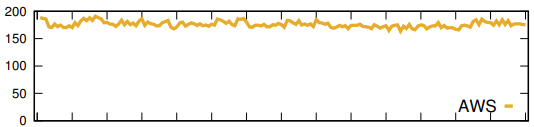
\includegraphics[width=1\textwidth]{images/lambda_cold_start.png}
    \caption{Latenza introdotta dal Cold Start (in ms) nell'arco di 168 ore. La prima invocazione richiede l'inizializzazione del runtime [Fonte: Wang et al., 2018]}
    \label{fig:lambda_cold_start}
\end{figure}

\subsection{Gestione delle API: Amazon API Gateway}
Amazon API Gateway funge da interfaccia per l'esposizione di API su protocollo HTTP/HTTPS, indirizzando le richieste client verso i servizi backend. Le funzionalità principali includono il controllo degli accessi, la limitazione della frequenza delle richieste (throttling) e il monitoraggio del traffico.
L'integrazione tramite Lambda Proxy demanda la formattazione della richiesta e della risposta direttamente alla funzione Lambda associata, semplificando la topologia di instradamento \cite{APIGatewayDoc}.

\subsection{Orchestrazione Eventi e Scheduling: Amazon EventBridge}
L'integrazione tra microservizi asincroni richiede un sistema di messaggistica affidabile. Amazon EventBridge è un bus di eventi che orchestra la comunicazione tra applicazioni e servizi AWS. Esso implementa anche meccanismi di pianificazione, abilitando l'esecuzione di funzioni Lambda a intervalli regolari. Questa caratteristica è essenziale per automatizzare l'avvio di pipeline di estrazione, trasformazione e caricamento (ETL) e processi batch \cite{EventBridgeDoc}.

\begin{figure}[ht!]
    \centering
    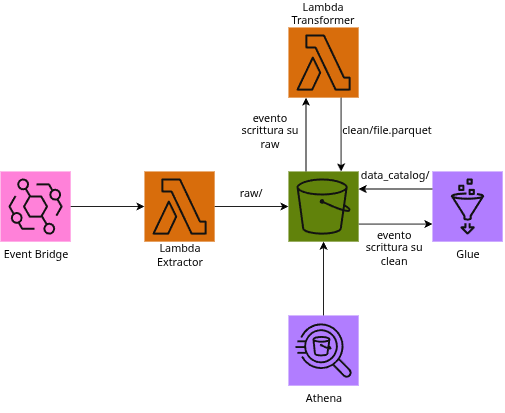
\includegraphics[width=1\textwidth]{images/pipeline-etl.drawio.png}
    \caption{Topologia di una pipeline ETL Serverless. Il flusso evidenzia l'estrazione da S3, la trasformazione via AWS Glue e l'esposizione per l'interrogazione tramite Amazon Athena [Elaborazione dell'autore]}
    \label{fig:pipeline-etl}
\end{figure}

\subsection{Messaggistica Asincrona e Pattern Publish-Subscribe: Amazon SNS}
\label{subsec:sns_dlq}

Nelle architetture a microservizi guidate da eventi, il disaccoppiamento tra i componenti produttori di dati e i componenti consumatori rappresenta un requisito primario per garantire la scalabilità indipendente. Tale disaccoppiamento è tipicamente implementato attraverso il pattern architetturale Publish-Subscribe (Pub/Sub) \cite{PubSubPattern}.

All'interno della piattaforma cloud in esame, questo pattern è concretizzato tramite Amazon Simple Notification Service (SNS). SNS opera come un servizio di messaggistica distribuito che facilita l'invio di messaggi (eventi) da un singolo applicativo (publisher) verso molteplici destinazioni (subscriber) in modalità asincrona. L'entità logica centrale è il \emph{topic}, un canale di comunicazione a cui i publisher inviano i messaggi e a cui i subscriber, come ad esempio funzioni AWS Lambda o endpoint HTTP, si registrano per riceverli \cite{SNS}. Questa configurazione abilita il \emph{fan-out} architetturale: un singolo evento innesca parallelamente molteplici flussi di elaborazione indipendenti, senza che il sistema originario debba gestire la logica di smistamento o conoscere a priori l'identità dei destinatari.

\subsection{Container Registry: Amazon ECR}
Le prassi standard di deployment prevedono l'utilizzo di immagini conformi alle specifiche OCI (Open Container Initiative) per incapsulare il software e le relative dipendenze. Amazon Elastic Container Registry (ECR) ospita le immagini Docker destinate all'esecuzione su AWS Lambda. Questo approccio sfrutta la memorizzazione nella cache dei livelli dell'immagine per ottimizzare i tempi di rilascio e permette l'inclusione di librerie scientifiche complesse, aggirando i limiti dimensionali dei tradizionali pacchetti compressi \cite{ECR}.

\subsection{Gestione della persistenza: Amazon DynamoDB e S3}
La natura stateless delle funzioni Lambda impone l'adozione di sistemi di persistenza in grado di supportare l'elevata concorrenza generata dal livello di calcolo. L'architettura fa affidamento su due soluzioni distinte.
La prima soluzione è Amazon DynamoDB, un database NoSQL di tipo chiave-valore. A differenza dei database relazionali, DynamoDB implementa uno scaling orizzontale, garantendo latenze ridotte anche durante i picchi di traffico. L'utilizzo di questo servizio implica la progettazione di schemi dati specifici, come il Single Table Design, per ottimizzare i percorsi di lettura e scrittura \cite{DynamoDBPaper}.

La seconda soluzione per la persistenza è Amazon S3, un servizio di archiviazione a oggetti. Esso assolve la funzione di repository per i dati non strutturati e agisce come livello di storage persistente per l'implementazione del Data Lake aziendale \cite{S3Doc}.

\subsection{Integrazione Dati: AWS Glue e Amazon Athena}
L'elaborazione dei dati all'interno del sistema richiede l'implementazione di pipeline ETL, il cui scopo è estrarre dati grezzi, trasformarli in formati analitici e caricarli nelle destinazioni finali. A tal fine, vengono impiegati due servizi cooperanti.
Il primo componente è AWS Glue, utilizzato nel sistema principalmente come Data Catalog. In questa architettura, il servizio non viene impiegato per l'esecuzione di cluster Spark \cite{Spark} distribuiti, bensì per il mantenimento di un catalogo di metadati centralizzato che descrive la struttura dei file Parquet \cite{Parquet} depositati nelle zone di archiviazione. L'operatore definisce tramite Glue gli schemi delle tabelle e la gerarchia delle partizioni temporali. Questo meccanismo permette al sistema di mappare i percorsi fisici su S3 verso entità logiche interrogate dai motori di calcolo superiori.
Il secondo componente è Amazon Athena, un motore di query interattivo basato su standard SQL che implementa il paradigma schema-on-read. Il servizio interroga direttamente il Data Catalog di Glue per risolvere la struttura dei dati e i predicati di partizionamento, senza la necessità di caricare preventivamente le informazioni in un database relazionale dedicato. Questa integrazione permette di eseguire analisi complesse sui dataset consolidati nel Data Lake, garantendo prestazioni elevate e una riduzione dei volumi di scansione tramite l'esclusione sistematica delle directory non pertinenti alla finestra temporale analizzata\cite{AWSGlueDoc}.

\subsection{Sicurezza, Identità e Controllo Accessi: IAM e Cognito}
In un'architettura distribuita basata su cloud, la sicurezza e l'isolamento delle risorse richiedono meccanismi di autenticazione e autorizzazione rigorosi, operanti a due livelli distinti: infrastrutturale e applicativo.

Il controllo degli accessi a livello infrastrutturale è governato da AWS Identity and Access Management (IAM). Questo servizio consente di definire in modo granulare quali entità (utenti umani, servizi o risorse di calcolo) dispongano delle autorizzazioni per invocare specifiche API cloud \cite{IAM}. La piattaforma in oggetto applica rigidamente il principio del privilegio minimo (Principle of Least Privilege): ogni microservizio, implementato tramite AWS Lambda, assume un ruolo IAM temporaneo dotato esclusivamente dei permessi strettamente necessari per l'esecuzione del proprio task, riducendo drasticamente la superficie di attacco \cite{LeastPrivilegeCloud}.

A livello applicativo, la gestione delle identità degli utenti finali è demandata ad Amazon Cognito, come illustrato in Figura \ref{fig:cognito-flow}. Cognito agisce come Identity Provider (IdP) e si integra nativamente con API Gateway per validare le richieste in ingresso. Al superamento delle credenziali, il servizio emette token aderenti allo standard JSON Web Token (JWT) \cite{JWT}. API Gateway intercetta questi token, ne verifica crittograficamente la firma e autorizza l'inoltro della richiesta al livello di calcolo sottostante, disaccoppiando così la logica di autenticazione dalla logica di business applicativa \cite{Cognito}.

\begin{figure}[ht!]
    \centering
    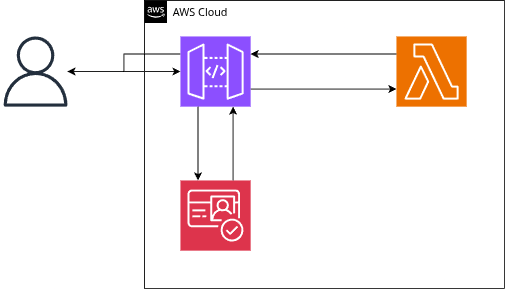
\includegraphics[width=1\textwidth]{images/cognito-api.drawio.png}
    \caption{Schema del flusso di comunicazione tra Api Gateway, Lambda e Cognito [Elaborazione dell'autore]}
    \label{fig:cognito-flow}
\end{figure}

\subsection{Osservabilità e Monitoraggio: Amazon CloudWatch}
La natura effimera e asincrona delle architetture Serverless rende inapplicabili i tradizionali approcci di debugging basati sull'accesso diretto ai server. Di conseguenza, l'osservabilità diviene un requisito architetturale primario per garantire la tracciabilità e la diagnostica del sistema \cite{ServerlessObservability}.

Il servizio Amazon CloudWatch costituisce il fulcro dell'infrastruttura di monitoraggio. Esso espleta tre funzioni essenziali: l'aggregazione centralizzata dei log generati dai container Lambda, la raccolta di metriche prestazionali (quali latenza di esecuzione, tasso di errore e consumo di memoria) e la gestione di allarmi automatizzati \cite{CloudWatch}. L'integrazione di CloudWatch garantisce agli operatori la visibilità sullo stato di salute dell'intero stack applicativo, fornendo i dati necessari per ottimizzare le risorse allocate e risolvere eventuali anomalie operative.

\subsection{Gestione Finanziaria e FinOps: AWS Cost Explorer}

Il paradigma del Cloud Computing trasforma le spese in conto capitale (CapEx) in spese operative (OpEx), introducendo un modello di fatturazione basato sul consumo effettivo (pay-as-you-go). In architetture ad alta densità di eventi, la frammentazione dei componenti serverless rende il monitoraggio finanziario un requisito ingegneristico fondamentale, inquadrato nella disciplina del Cloud Financial Management o FinOps \cite{FinOpsBook}.

L'analisi e l'ottimizzazione della spesa all'interno della piattaforma sono demandate ad AWS Cost Explorer. Questo servizio elabora i dati di telemetria finanziaria fornendo interfacce per la visualizzazione storica, l'identificazione delle anomalie e la previsione dei costi futuri \cite{CostExplorer}.

Un meccanismo essenziale per la ripartizione dei costi in ambienti complessi è costituito dai Cost Allocation Tags. Attraverso l'applicazione di metadati strutturati alle singole risorse infrastrutturali, Cost Explorer aggrega la spesa per dominio logico (ad esempio, per ambiente di rilascio, centro di costo o specifico microservizio). Questa aggregazione abilita il tracciamento granulare del costo per singola transazione e garantisce la tracciabilità economica dell'intero stack applicativo \cite{CostAllocationTags}.

\section{Sviluppo Applicativo: Servizi e Worker}
\label{sec:app_frameworks}

I microservizi sviluppati si dividono in due categorie funzionali: i servizi di backend che espongono API sincrone e i worker asincroni adibiti all'elaborazione dei dati.

\subsection{Sviluppo di Backend API con FastAPI}
La programmazione dei servizi API si avvale di Python, ampiamente adottato per lo sviluppo backend \cite{PythonTrends}, e del framework FastAPI. Oltre al supporto nativo per la concorrenza asincrona, FastAPI utilizza la libreria Pydantic per validare a runtime la struttura dei dati in ingresso e in uscita. Questo meccanismo previene gli errori legati alla tipizzazione e garantisce l'aderenza delle richieste ai formati attesi \cite{FastAPIDoc}. Il framework genera inoltre autonomamente la specifica OpenAPI, facilitando la documentazione delle interfacce.

\subsection{Elaborazione Asincrona: Event-Driven Workers}
A differenza dei servizi API, che seguono un paradigma richiesta-risposta sincrono, i worker operano in modalità totalmente asincrona e disaccoppiata, come illustrato nello schema in Figura \ref{fig:pipeline-etl}. In un'architettura guidata da eventi, un worker è un componente software incaricato di eseguire operazioni ad alta intensità computazionale o processi di background, quali le trasformazioni ETL (Extract, Transform, Load), la pulizia dei dati o la sincronizzazione con sistemi di terze parti.

L'esecuzione di un worker non è innescata da una chiamata HTTP diretta, bensì da eventi di sistema emessi dall'infrastruttura cloud. Tali eventi includono il caricamento di un oggetto in un bucket Amazon S3, la pubblicazione di un messaggio su un topic SNS, o lo scoccare di una regola cronologica definita in Amazon EventBridge. Questo radicale disaccoppiamento garantisce la scalabilità indipendente dei processi di elaborazione dati, impedendo che i carichi di lavoro intensivi saturino le risorse o aumentino la latenza delle interfacce esposte agli utenti \cite{EventDrivenArchitecture}.

\subsection{Adattamento al runtime Lambda: Mangum e Lambda RIC}
L'esecuzione del codice all'interno dell'ambiente AWS Lambda necessita di moduli di interfaccia specifici per colmare la differenza tra i protocolli standard e gli eventi proprietari del cloud provider.
Per i servizi API, viene utilizzato Mangum, come illustrato in Figura \ref{fig:mangum}. Questo adattatore converte i payload JSON forniti da API Gateway in richieste HTTP standardizzate, permettendo l'esecuzione di applicazioni conformi allo standard ASGI (come FastAPI) all'interno di Lambda \cite{MangumDoc}.
Per i worker asincroni, si impiega l'AWS Lambda Runtime Interface Client (RIC). Tale libreria espone l'API del runtime Lambda ai container Docker personalizzati, consentendo l'esecuzione di script Python generici in risposta a eventi non HTTP.

\begin{figure}[ht!]
    \centering
    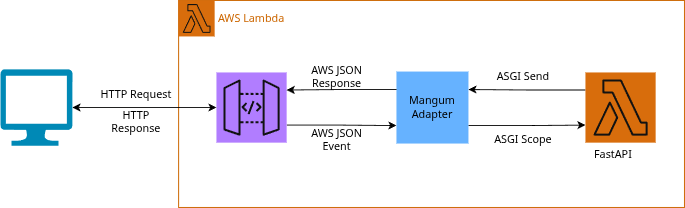
\includegraphics[width=1\textwidth]{images/mangum.drawio.png}
    \caption{Schema del flusso di adattamento tramite Mangum. L'evento AWS viene tradotto in una richiesta compatibile con l'interfaccia ASGI [Elaborazione dell'autore]}
    \label{fig:mangum}
\end{figure}

\section{Infrastructure as Code con Terraform}
\label{sec:terraform_iac}

La configurazione manuale tramite interfaccia grafica di infrastrutture complesse risulta soggetta a errori e non replicabile. L'approccio Infrastructure as Code (IaC) mitiga queste problematiche definendo l'infrastruttura tramite file di testo strutturati.

\subsection{Il paradigma dell'Infrastruttura Immutabile}
L'IaC abilita il controllo di versione per l'infrastruttura tramite Git \cite{Git}, assoggettandola ai medesimi processi di revisione del codice software. Strumenti come Terraform utilizzano un approccio dichiarativo: l'ingegnere specifica lo stato finale atteso per le risorse cloud, ed è responsabilità del software calcolare il piano di esecuzione e applicare le mutazioni necessarie per allineare l'ambiente reale alla configurazione definita \cite{IaCGuerriero}.

\subsection{Modularità e Gestione dello Stato}
Terraform mappa la configurazione dichiarata con le risorse allocate sul cloud attraverso un file di stato remoto. Al fine di standardizzare la creazione delle risorse ed evitare la duplicazione del codice, l'architettura fa ampio uso dei moduli Terraform. L'incapsulamento delle definizioni infrastrutturali all'interno di moduli riutilizzabili assicura che ogni nuovo servizio ereditato rispetti intrinsecamente i parametri di sicurezza e di tracciamento aziendali \cite{TerraformUpAndRunning}.

\subsection{Orchestrazione dell'Infrastruttura e principio DRY: Terragrunt}

La gestione di architetture multi-ambiente tramite il solo framework Terraform impone la replicazione del codice dichiarativo per ogni contesto di esecuzione, incrementando il debito tecnico. Per risolvere questa limitazione strutturale, l'architettura si avvale di Terragrunt. Terragrunt è un orchestratore open-source che agisce come livello di astrazione (wrapper) superiore rispetto all'eseguibile nativo di Terraform. Il software intercetta i comandi operativi impartiti dall'utente e inietta dinamicamente i parametri di configurazione prima di delegarne l'esecuzione al motore di provisioning sottostante.

L'adozione di questo orchestratore abilita l'applicazione rigorosa del principio ingegneristico Don't Repeat Yourself. L'ingegnere definisce la logica di creazione delle risorse una singola volta all'interno di moduli Terraform generici e isolati. Successivamente, tramite i file di configurazione proprietari di Terragrunt, il sistema instaura delle gerarchie di ereditarietà. Le directory che mappano gli ambienti fisici (come lo sviluppo o la produzione) si limitano a ereditare la logica del modulo base, sovrascrivendo unicamente le variabili specifiche del contesto, quali il dimensionamento computazionale o i puntamenti di rete.

Oltre alla deduplicazione del codice, l'orchestratore automatizza la gestione dello stato remoto (remote state). Terragrunt genera e configura dinamicamente i backend di archiviazione per ogni singolo ambiente, prevenendo errori di configurazione manuale che causerebbero la corruzione dello stato infrastrutturale. Questa standardizzazione assicura che i file di stato rimangano rigorosamente segregati per ciascun account cloud aziendale.

Infine, il framework introduce costrutti dichiarativi espliciti per la risoluzione delle dipendenze inter-modulo. Terraform nativamente non permette di orchestrare moduli situati in directory distinte; Terragrunt supera questo ostacolo calcolando il grafo topologico dell'intera infrastruttura. Questa funzionalità permette al sistema di passare le variabili di output di un modulo (come l'identificativo di una rete appena creata) come parametri di input per un modulo dipendente (come un cluster di calcolo), garantendo il rispetto della corretta sequenza logica durante le operazioni di rilascio. \cite{Terragrunt}

\section{Automazione del Ciclo di Vita del Software (SDLC)}
\label{sec:sdlc}

L'automazione del ciclo di sviluppo (SDLC) si prefigge di ottimizzare l'iterazione tra la stesura del codice, la sua validazione e la successiva messa in produzione.

\subsection{Containerizzazione e parità degli ambienti}
La distribuzione del codice tramite archivi compressi comporta limitazioni operative, quali la difficoltà di includere librerie pre-compilate e l'impossibilità di garantire l'identità tra l'ambiente di sviluppo e quello di esecuzione. L'adozione dello standard Docker permette di incapsulare l'applicativo, le librerie e il sistema operativo di base all'interno di un'immagine immutabile. Questo garantisce la parità degli ambienti, assicurando che il comportamento del software validato localmente dallo sviluppatore rimanga coerente una volta rilasciato nell'infrastruttura di produzione \cite{DockerDoc}.

\subsection{Emulazione Cloud per lo sviluppo locale: LocalStack}
Un ostacolo intrinseco allo sviluppo di applicazioni Cloud-Native è la latenza introdotta dalla necessità di distribuire ogni singola modifica sull'infrastruttura remota per poterne verificare il funzionamento. Questa dipendenza dilata i tempi del ciclo di iterazione locale, definito come la sequenza di scrittura, compilazione e test del codice \cite{RedHatInnerLoop}.
Per ripristinare un ciclo di sviluppo rapido, viene impiegato LocalStack, un emulatore che espone API compatibili con i principali servizi AWS. L'esecuzione di LocalStack tramite container permette di simulare l'interazione tra componenti come Lambda, DynamoDB e S3 direttamente sulla postazione di lavoro, abilitando il collaudo del software in assenza di connettività verso il cloud e abbattendo i tempi di attesa \cite{LocalStackPaper}.

\subsection{Continuous Integration e Delivery (CI/CD)}
Le pratiche di Continuous Integration e Continuous Delivery automatizzano le fasi di test e rilascio. Tramite piattaforme come GitHub Actions, il caricamento di nuovo codice sorgente innesca l'esecuzione sequenziale di test unitari, la compilazione delle immagini Docker e il caricamento sul registro ECR. Questo flusso di lavoro automatizzato esclude le operazioni manuali dai processi di deployment, garantendo la riproducibilità tecnica dei rilasci \cite{AccelerateBook}.

\section{Evoluzione dell'Automazione: LLM e Model Context Protocol}
\label{sec:mcp_background}

La recente diffusione dei Large Language Models (LLM) ha introdotto nuovi paradigmi nell'ambito dell'ingegneria del software, estendendo le capacità di automazione oltre la generazione statica di codice \cite{LLMSoftwareEngineering}. Tuttavia, l'efficacia di tali modelli in contesti aziendali è storicamente limitata dal loro isolamento rispetto agli ambienti di esecuzione locali e alle infrastrutture proprietarie.

Per superare tale limitazione, la letteratura tecnica ha formalizzato il concetto di \textit{Tool Use} (o \textit{Function Calling}), ovvero la capacità di un modello di delegare l'esecuzione di calcoli deterministici o l'interazione con sistemi esterni a script predefiniti \cite{LLMTool}.
In questo contesto si inserisce il Model Context Protocol (MCP), uno standard aperto introdotto per uniformare la comunicazione tra le applicazioni di intelligenza artificiale (Client) e le sorgenti di dati o gli strumenti operativi (Server) \cite{MCP}.

Il protocollo MCP adotta un'architettura client-server standardizzata, definendo un insieme rigoroso di primitive per l'esposizione di risorse, prompt e strumenti (Tools). Tale astrazione permette agli ambienti di sviluppo integrati (IDE) dotati di agenti conversazionali di interrogare un server MCP locale o remoto per scoprire quali operazioni infrastrutturali siano disponibili, ottenendo in risposta il relativo schema JSON dei parametri richiesti.
Al fine di accelerare lo sviluppo di server compatibili con tale standard, l'ecosistema Python mette a disposizione librerie come FastMCP \cite{FastMCP}. Questi framework astraggono la complessità del trasporto a basso livello (gestito tipicamente tramite stdio o Server-Sent Events), consentendo all'ingegnere di mappare le funzioni Python direttamente sulle interfacce del protocollo tramite l'impiego di decoratori sintattici, garantendo la validazione automatica dei tipi in ingresso e in uscita.

\begin{figure}[ht!]
    \centering
    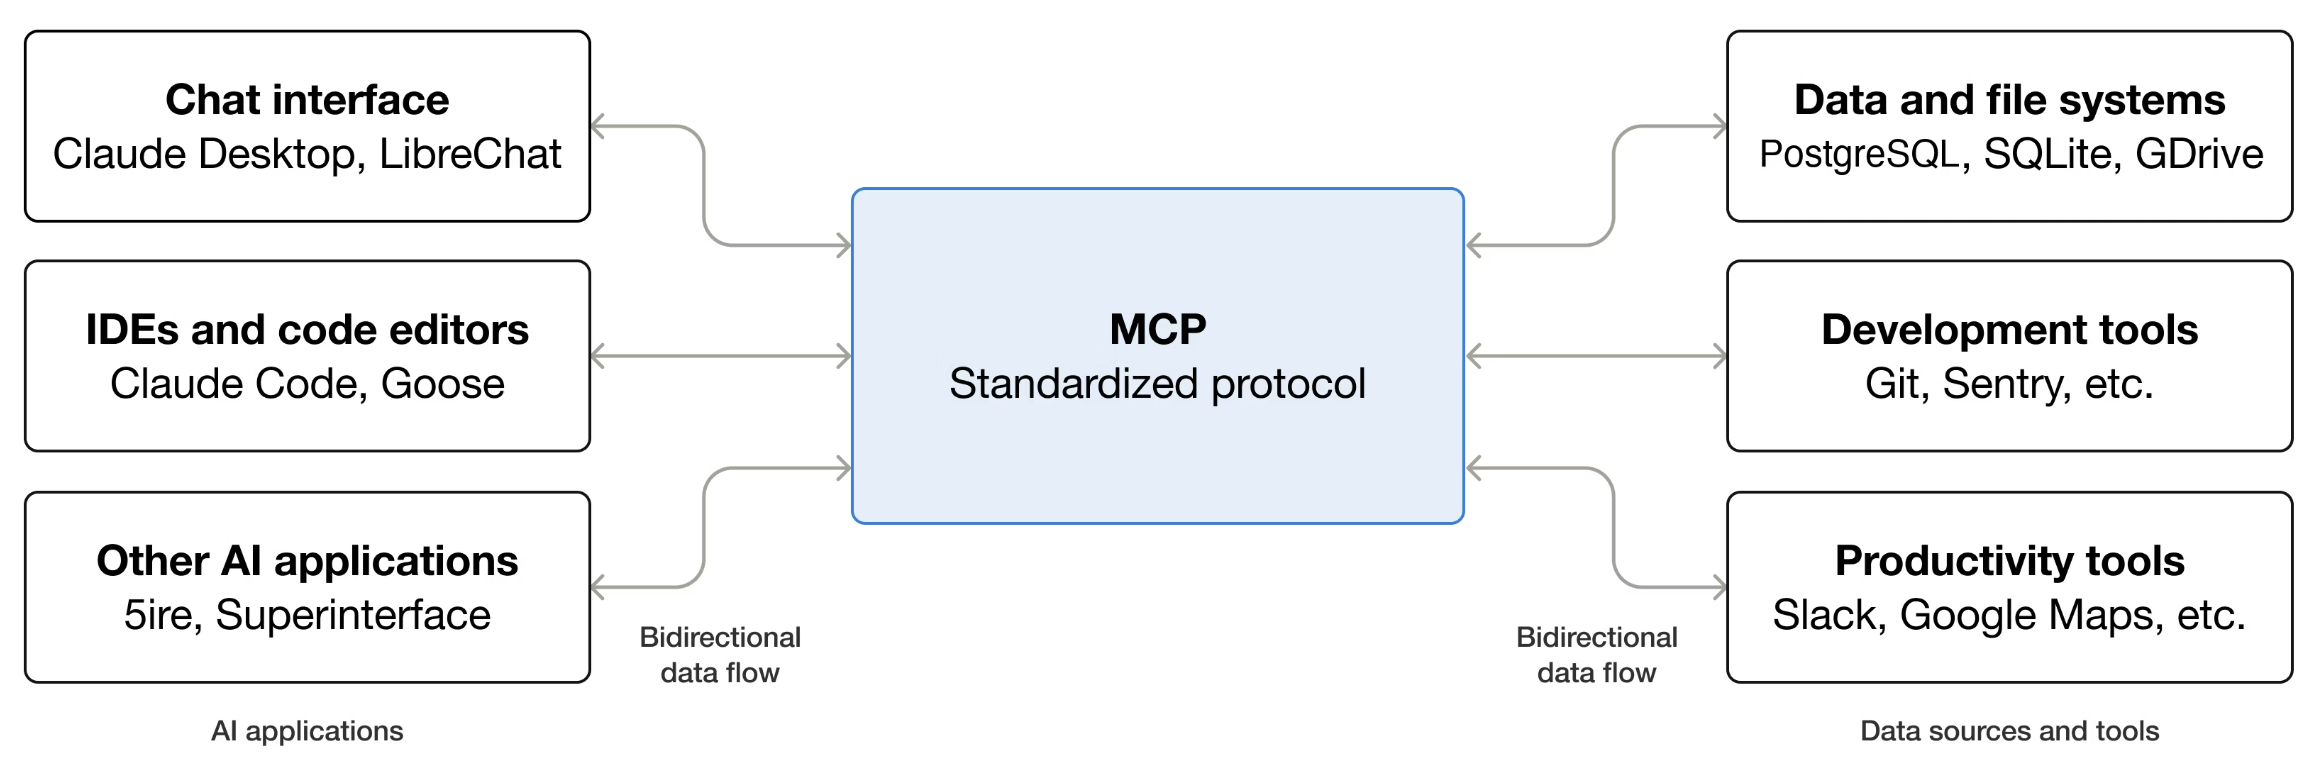
\includegraphics[width=1\textwidth]{images/mcp.png}
    \caption{MCP come protocollo di comunicazione standard tra LLM e tools [Fonte: modelcontextprotocol.io \cite{MCP}]}
    \label{fig:mcp}
\end{figure}